\clearpage

\section{X. Программа экзамена в 2024/2025}


\begin{enumerate}
    \item Выборочная функция распределения. Теоремы Гливенко-Кантелли и Колмогорова.

    \Def \hyperlink{selective_distribution_function}{Выборочной функцией распределения} $F^*(x)$ называется функция $F^*(x) = \frac{\text{число данных } x_i < x}{n}$

    \begin{MyTheorem}
        \Ths Выборочная функция распределения поточечно сходится к теоретической функции распределения:

        \[\forall y \in \Real F^*(y) \overset{p}{\longrightarrow} F(y)\]
    \end{MyTheorem}

    \begin{MyTheorem}
        \ThNs{Гливенко-Кантелли} $\sup_{x \in \Real} |F^*(x) - F(x)| \overset{p}{\longrightarrow} 0$
    \end{MyTheorem}

    \begin{MyTheorem}
        \ThNs{Колмогорова} $\sqrt{n} \sup_{x \in \Real} |F^*(x) - F(x)| \rightrightarrows K$ - распределение Колмогорова с 
        функцией распределения $F_K(x) = \sum_{j = -\infty}^{\infty} (-1)^j e^{-2 j^2 x^2}, \ x \in [0;\infty)$
    \end{MyTheorem}

    \item Вариационный и интервальный вариационный ряды. Полигон и гистограмма, ее свойства.

        
    \hyperlink{initial_data_processing}{Начальная обработка статданных}

    \begin{enumerate}
        \item Ранжирование данных - упорядочиваем выборки по возрастанию. В результате получаем вариационный ряд $\vec{X} = (X_{(1)}, X_{(2)}, \dots, X_{(n)})$

        $X_{(1)} = \min X_i; \quad X_{(n)} = \max X_i$

        $X_{(i)} = i$-ая порядковая статистика

        \item Объединим повторяющиеся данные - получаем т.н. частотный вариационный ряд

        \begin{tabular}{c|c|c|c|c}
            $X_i$ & $X_{(1)}$ & \dots & $X_{(r)}$ & $\sum$ \\ 
            \hline
            $n_i$ & $n_1$ & \dots & $n_r$ & $n$ \\ 
        \end{tabular}

        Иногда часть данных отбрасывается сверху и снизу (по 5, по 10, по 5\% и так далее), чтобы сделать выборку репрезентативной

        Тогда $\overline{x} = \frac{1}{n} \sum X_i n_i$, $D^* = \frac{1}{n} \sum (X_i - \overline{x})^2 n_i$
        
        \item Чтобы уменьшить количество вычислений или сделать гистограмму, делают интервальный вариационный ряд: 
        разбиваем данные на интервалы и считаем, сколько данных $n_i$ попало в интервал. 

        Тогда $n_i$ - частота интервала $A_i$

        Есть два основные способа разбиения на интервалы: 

        \begin{enumerate}
            \item Интервалы одинаковой длины
            \item Равнонаполненные интервалы (в каждом интервале примерно одинаковое количество данных)
        \end{enumerate}

        Число интервалов $K$ такое, что $\frac{K(n)}{n} \longrightarrow 0$ и $K(n) \underset{n \to \infty}{\longrightarrow} \infty$

        Обычно применяют формулу Стерджесса $K \approx 1 + \log_2 n$ или $K \approx \sqrt[3]{n}$

        Пусть получили интервальный вариационный ряд

        \begin{tabular}{c|c|c|c|c|c}
            интервалы & $[a_0; a_1)$ & $[a_1; a_2)$ & \dots & $[a_{K - 1}; a_K]$ & $\sum$ \\ 
            \hline
            частоты & $n_1$ & $n_2$ & \dots & $n_K$ & $n$ \\ 
        \end{tabular}
    \end{enumerate}

    \smallvspace
        
    \begin{multicols}{2}
        \begin{itemize}
            \item Гистограмма

            Строится ступенчатая фигура из прямоугольников, основание $i$-ого прямоугольника - интервал, 
            высота прямоугольника - $\frac{n_i}{n l_i}$, где $l_i$ - длина интервала. 
            Визуально можно сделать гипотезу, как ведет себя распределение. 

            \begin{center}
                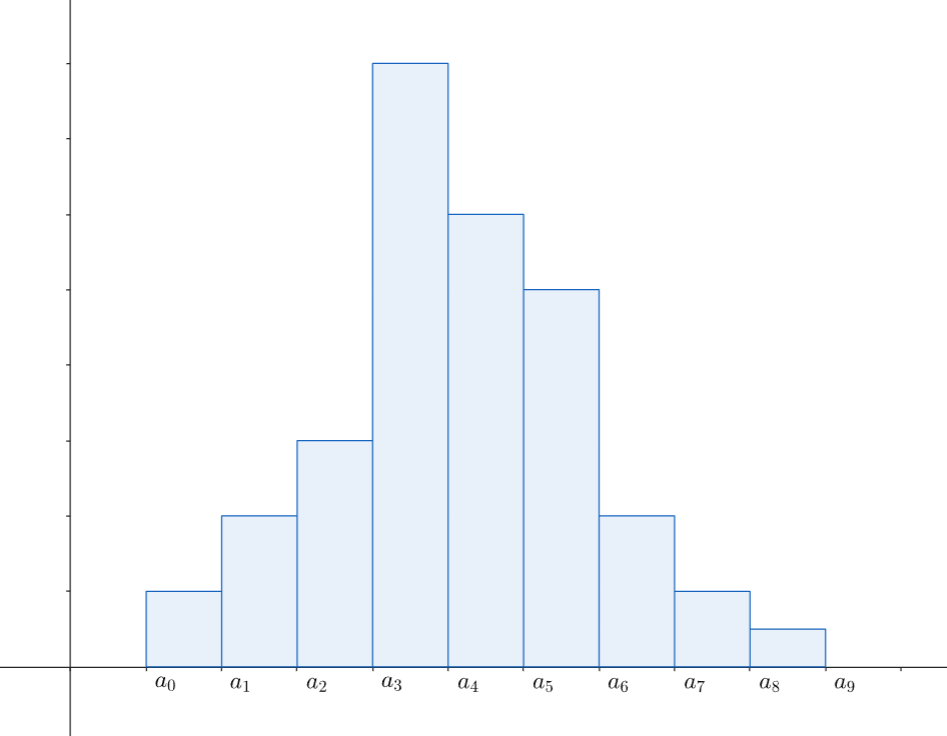
\includegraphics[width=0.4\textwidth]{mathstat/images/mathstat_2025_02_11_1}
            \end{center}

            \item Полигон

            На оси абсцисс отмечаем значения частотного вариационного ряда, по оси ординат - их частоты. 
            Получившиеся точки соединяем отрезками

            \begin{center}
                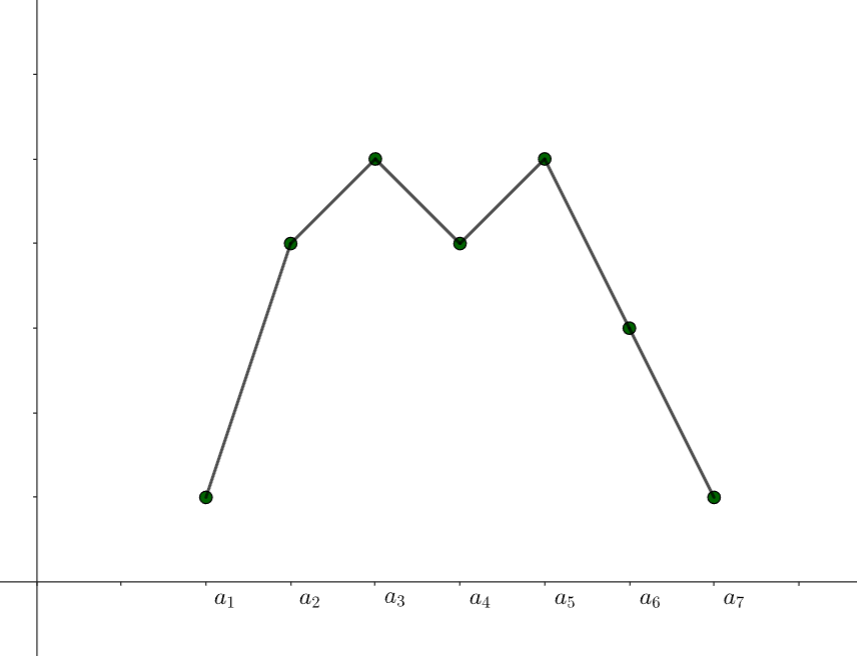
\includegraphics[width=0.4\textwidth]{mathstat/images/mathstat_2025_02_11_2}
            \end{center}
        \end{itemize}
    \end{multicols}


    \item Точечные оценки. Их свойства: состоятельность, несмещенность, эффективность.
    \item Точечные оценки моментов. Свойства оценок математического ожидания и дисперсии.
    \item Метод моментов. Пример.
    \item Метод максимального правдоподобия. Пример.
    \item Информация Фишера. Неравенство Рао-Крамера (без док-ва).
    \item Основные распределения математической статистики: хи-квадрат, Стьюдента, Фишера-Снедекора. Их свойства.
    \item Линейные преобразования нормальных выборок. Теорема об ортогональном преобразовании.
    \item Лемма Фишера.
    \item Основная теорема о связи точечных оценок нормального распределения и основных распределений статистики.
    \item Квантили распределений (оба определения). Функции для их вычисления в EXEL.
    \item Интервальные оценки. Определения, смысл, терминология.
    \item Доверительный интервал для математического ожидания нормального распределения при известном σ.
    \item Доверительный интервал для математического ожидания нормального распределения при неизвестном σ.
    \item Доверительный интервал для дисперсии нормального распределения при неизвестном a.
    \item Доверительный интервал для дисперсии нормального распределения при известном a.
    \item Проверка статистических гипотез. Определения, терминология. Уровень значимости и мощность критерия.
    \item Способы сравнения критериев проверки гипотез.
    \item Построение критериев согласия (основные принципы).
    \item Гипотеза о среднем нормальной совокупности с известной дисперсией.
    \item Гипотеза о среднем нормальной совокупности с неизвестной дисперсией.
    \item Доверительные интервалы как критерии гипотез о параметрах распределения.
    \item Критерий хи-квадрат для параметрической гипотезы.
    \item Критерий хи-квадрат для гипотезы о распределении.
    \item Критерий Колмогорова для гипотезы о распределении.
    \item Критерий Колмогорова-Смирнова.
    \item Критерий Фишера.
    \item Критерий Стьюдента.
    \item Понятие статистической зависимости. Корреляционное облако и корреляционная таблица. Первоначальные выводы.
    \item Критерий хи-квадрат для проверки независимости.
    \item Однофакторный дисперсионный анализ. Общая, межгрупповая и внутригрупповая дисперсии. Теорема о разложении дисперсии.
    \item Однофакторный дисперсионный анализ. Проверка гипотезы о влиянии фактора.
    \item Математическая модель регрессии. Основные понятия и определения. Метод наименьших квадратов.
    \item Вывод уравнения линейной парной регрессии. Геометрический смысл прямой регрессии.
    \item Выборочный коэффициент линейной корреляции. Проверка гипотезы о его значимости.
    \item Выборочное корреляционное отношение, его свойства.
    \item Свойства ошибок в модели линейной парной регрессии. Анализ дисперсии фактора-результата. Коэффициент детерминации, его свойства.
    \item Проверка гипотезы о значимости уравнения линейной регрессии. Связь между коэффициентом детерминации и коэффициентом линейной корреляции.
    \item Теорема Гаусса-Маркова.
    \item Стандартные ошибки коэффициентов регрессии. Их доверительные интервалы.
    \item Прогнозирование в модели линейной парной регрессии. Стандартная ошибка прогноза, доверительный интервал прогноза.
    \item Общая модель линейной регрессии. Вывод нормального уравнения.
    \item Свойства ОНМК в уравнении общей линейной регрессии.
    \item Основная теорема об ОМНК (п.2 без доказательства).
    \item Мультиколлинеарность, ее неприятные последствия. Основные принципы отбора факторов в модель общей линейной регрессии.
    \item Стандартная ошибка общей линейной регрессии и стандартные ошибки коэффициентов регрессии. Проверка гипотезы о значимости отдельного коэффициента регрессии.
    \item Уравнение регрессии в стандартных масштабах. Смысл стандартизованных коэффициентов. Разложение влияния фактора на прямое и косвенное.
    \item Коэффициенты детерминации и множественной корреляции, их свойства. Проверка гипотезы о значимости уравнения регрессии в целом.
    \item Взвешенный МНК.
    \item Приемы сведения нелинейных регрессий к линейным.
    \item Математические датчики случайных чисел.
    \item Моделирование случайных величин методом обратной функции (включая дискретный случай).
    \item Моделирование нормальной случайной величины.
    \item Быстрый показательный датчик.
    \item Моделирование дискретных случайных величин.
    \item Метод Монте-Карло. Общая постановка, оценка погрешности.
    \item Вычисление определенного и кратного интегралов методом Монте-Карло. Метод расслоенной выборки.
\end{enumerate}
